\documentclass[../../manuale-manutentore.tex]{subfiles}

\begin{document}
\subsection{Mobile app}%
\label{sub:mobile_app}

Tutte le classi definite per l'applicazione mobile sono raccolte nel package \java{tech.gruppone.stalker.app}, i cui subpackage sono organizzati come indicato in figura §\ref{fig:app/diagramma_package}
\begin{figure}[ht]
  \centering
  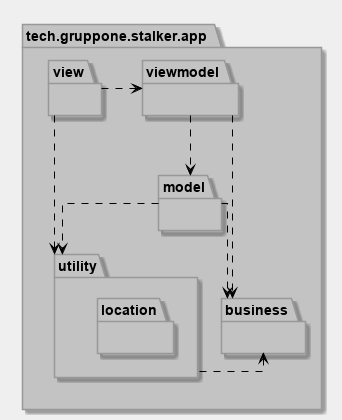
\includegraphics[width=6cm]{app-package-diagram.png}
  \caption{Diagramma dei package per l'applicazione mobile}
~~\label{fig:app/diagramma_package}
\end{figure}

\subsubsection{MVVM}%
\label{subs:mvvm}

Per la mobile app abbiamo scelto il pattern Model-View-ViewModel, in quanto è supportato nativamente dalle librerie di Android e si integra perfettamente con il sistema di \glossarioLocale{lifetime} del framework. Per ogni schermata \textit{X} visualizzata dall'utente, ad esempio la schermata di \textit{Login}, sono individuate:
\begin{itemize}
  \item Una classe \java{XActivity} derivata da \java{androidx.appcompat.app.AppCompActivity}, corrispondente alla View, a cui è associato un \glossarioLocale{layout} \linebreak[1]\texttt{activity\_x.xml} scritto in XML\@.
  \item Se necessario, una classe \java{XViewModel} derivata da \java{androidx.lifecycle.ViewModel} corrispondente al ViewModel.
  \item Se necessario, una classe \java{XModel} derivata da \java{java.lang.Object} corrispondente al Model.
\end{itemize}

GruppOne raccoglie le classi \java{XActivity}, \java{XViewModel} e \java{XModel} rispettivamente nei subpackage \java{view}, \java{viewmodel} e \java{model}.
Le tre classi formano la gerarchia mostrata in figura §\ref{fig:app/diagramma_classi_mvvm}.
Mentre \java{XViewModel} può semplicemente istanziare \java{Model}, \java{XActivity} deve ricevere un'istanza di \java{XViewModel} da un \java{androidx.lifecycle.ViewModelProvider} attraverso il metodo \java{get(Class<T>)}, a causa del lifetime system.
Ogni volta che un oggetto associato alla stessa schermata, e quindi istanza della stessa classe \java{XActivity}, viene costruito, ad esempio dopo che lo schermo è stato ruotato, il \java{ViewModelProvider} gli restituisce la stessa istanza della classe \java{XViewModel}.
Il modo più comune di ottenere l'istanza di \java{XViewModel}, a meno degli opportuni \java{import}, è:

\begin{minted}{java}
class XActivity extends AppCompActivity {
  ...
  private XViewModel viewModel;

  @Override
  protected void onCreate(@Nullable Bundle savedInstanceState) {
    ...
    viewModel = new ViewModelProvider(this).get(XViewModel.class);
    ...
  }
  ...
}
\end{minted}

Siccome i permessi di geolocalizzazione sono necessari al corretto funzionamento dell'applicazione, essa verifica ogni volta che viene aperta o riportata in primo piano che non siano stati revocati.
Per questo abbiamo scelto di utilizzare un decorator pattern, quindi forniamo la classe \java{utility.StalkerActivity} come classe derivata da \java{androidx.appcompat.app.AppCompatActivity} per eseguire automaticamente questa verifica.

\begin{figure}[ht]
  \centering
  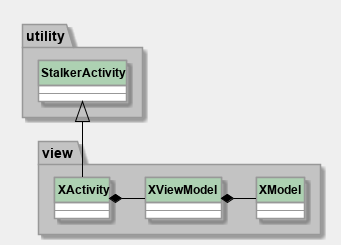
\includegraphics{app-mvvm.png}
  \caption{Diagramma delle classi per MVVM}
~~\label{fig:app/diagramma_classi_mvvm}
\end{figure}

Per quanto riguarda l'autenticazione, e quindi le schermate di \textit{Login} e \textit{Signup}, il viewmodel ha la responsabilità di produrre un hash della password, mentre il model ha la responsabilità di definire il metodo \glossarioLocale{callback} che viene invocato quando il server risponde alla richiesta.

\subsubsection{Pagina principale}%
\label{subs:pagina_principale}

La pagina principale utilizza tre fragment per mostrare all'utente le liste di organizzazioni a cui può connettersi e a cui è connesso, e il report della propria cronologia.
Ciascun fragment rispetta il pattern MVVM, e le rispettive classi fragment stesso, viewmodel e model sono raccolte nei subpackage \java{view.fragment}, \java{viewmodel.fragment} e \java{model.fragment}.

% subs:pagina_principale (end)

\subsubsection{Pagina organizzazione}%
\label{subs:pagina_organizzazione}
Da una delle liste di organizzazioni, è possibile accedere alla pagina specifica di un'organizzazione toccando il rispettivo elemento nell'elenco.
La pagina sfrutta le \textit{Maps API} di Google per mostrare una mappa con una rappresentazione dei luoghi monitorati dall'organizzazione attraverso dei poligoni colorati.
Il rispettivo viewmodel ha la responsabilità di raccogliere le informazioni di dettaglio dell'organizzazione da mostrare, ed elaborarle perché siano direttamente utilizzabili dall'activity.

% subs:pagina_organizzazione (end)

\subsubsection{RecyclerView}%
\label{subs:recyclerview}

I fragment della schermata principale mostrano liste che si devono aggiornare dinamicamente per mostrare all'utente dei dati sempre aggiornati.
A questo scopo abbiamo scelto di utilizzare \java{androidx.recyclerview.widget.RecyclerView}, componente grafica che astrae il confronto fra la lista nuova e quella attuale, richiedendo un minimo quantitativo di codice per specificare come confrontare gli elementi uno ad uno.
Questo deve essere fornito nella forma di un'istanza di una classe derivata da \java{androidx.recyclerview.widget.ListAdapter}, una classe generica con due parametri di tipo.
A questo scopo, GruppOne ha definito la classe \java{OrganizationListAdapter} nel subpackage \java{view.recyclerview}.
Per l'estensione di \java{ListAdapter} il primo parametro di tipo deve essere sostituito con il tipo degli oggetti nella lista, nel nostro caso \java{business.Organization} (§\ref{subs:logica_di_business}), il secondo con una classe derivata da \java{RecyclerView.ViewHolder}.
Quest'ultima rappresenta un elemento della lista e racchiude metadati sulla sua posizione; ciascun \java{ListAdapter} istanzia e modifica i \java{ViewHolder} a propria necessità per aggiornare la \java{Recyclerview}, quindi essi sono da considerarsi come semplici frammenti della funzionalità del \java{ListAdapter} stesso.
Di conseguenza, la nostra estensione di \java{ViewHolder}, \java{OrgViewHolder}, è innestata nella classe \java{OrganizationListAdapter}. Ogni estensione di \java{ViewHolder} deve essere associata ad un layout XML che descriva la grafica del rispettivo elemento nella lista.\par

Ogni estensione di \java{ListAdapter} deve fornire al costruttore della superclasse un'istanza di \linebreak\java{androidx.recyclerview.widget.DiffUtil.ItemCallback} che definisca metodi per confrontare un elemento della lista nuova con il corrispondente nella lista già presente e verificare se coincidono oppure se non coincidono ma sono comunque equivalenti. Inoltre deve fornire override per i metodi:
\begin{itemize}
  \item\java{public OrgViewHolder onCreateViewHolder(ViewGroup parent, int viewType)}, che deve costruire un \java{ViewHolder} appropriato al contesto grafico, dato da \java{parent}, e della tipologia indicata da \java{viewType}.
  \item\java{public void onBindViewHolder(OrgViewHolder holder, int position)}, che deve eseguire tutte le operazioni necessarie affinché \java{holder} rappresenti correttamente l'elemento in lista alla posizione \java{position}.
  \item\java{public int getItemViewType(int position)}, che deve ritornare la tipologia di \java{ViewHolder} associata alla posizione  \java{position}. In particolare, questo metodo è utile per differenziare ad esempio gli elementi pari dai dispari, e generalmente ritorna una delle costanti definite in \java{R.layout} corrispondenti ai layout associati alle estensioni di \java{ViewHolder}.
\end{itemize}

Le estensioni di \java{ViewHolder} non hanno requisiti rigidi, ma preferibilmente dovrebbero prevedere una cache di riferimenti ad elementi grafici di cui fanno uso, per limitare il numero di chiamate a \java{findViewById(int)}, le quali potrebbero rallentare l'applicazione.

\paragraph{Selezione di elementi}%
\label{par:selezione_di_elementi}
Attraverso \java{recyclerview-select}, un'estensione della libreria \java{recyclerview}, è possibile selezionare gli elementi delle liste per effettuare operazioni batch, come collegarsi e scollegarsi contemporaneamente da più organizzazioni.
Tutte le classi necessarie ad implementare questa funzionalità sono raccolte nel subpackage \java{view.recyclerview}.
La classe fondamentale per gestire la selezione è \linebreak\java{androidx.recyclerview.selection.SelectionTracker}, che sfrutta un'associazione fra un insieme di chiavi e gli elementi della lista per monitorare quali elementi sono selezionati.
Il suo builder richiede come parametri:
\begin{itemize}
  \item la recyclerview da monitorare
  \item un'istanza di \java{androidx.recyclerview.selection.ItemKeyProvider} che permette di ottenere la chiave di un elemento data la sua posizione nell'elenco e viceversa
  \item un'istanza di \linebreak\java{androidx.recyclerview.selection.ItemDetailsLookup} che permette di ricavare i dettagli dell'elemento selezionato a partire dall'evento scatenato dall'interazione con l'utente
  \item un'istanza di \java{androidx.recyclerview.selection.StorageStrategy} che permette di serializzare le chiavi
\end{itemize}

Inoltre è necessario fornire un'istanza di \java{SelectionTracker.SelectionPredicate}, che permette di disabilitare la selezione per elementi date le rispettive chiavi.
Abbiamo utilizzato la classe derivata \java{OnlyPublicSelectionPredicate} per impedire la selezione di organizzazioni private nel caso della connessione, per evitare la confusione di dover inserire più credenziali LDAP alla volta.
Per reagire alla selezione è necessario aggiungere al \java{SelectionTracker} un \java{SelectionTracker.SelectionObserver}.
Il suo metodo \java{onSelectionChanged()} distingue i vari casi (primo elemento selezionato, ultimo elemento deselezionato, caso generico) attraverso dei controlli sul numero di elementi selezionati e sullo stato di attivazione della action bar dell'activity.
In particolare, quando ci sono elementi selezionati, la action bar viene sostituita da una context bar, che permette di eliminare la selezione oppure di eseguire l'operazione batch (connessione o disconnessione) su tutti gli elementi selezionati.

% par:selezione_di_elementi (end)

\paragraph{Integrazione con MVVM}%
\label{par:integrazione_con_mvvm}

Il \java{ListAdapter} riceve la nuova lista, con la quale aggiornare la \java{RecyclerView}, attraverso il metodo \linebreak\java{submitList(List<T>)}.
La lista di organizzazioni viene aggiornata attraverso una richiesta HTTP al server (§\ref{subs:richieste_http}), la quale viene gestita in modo asincrono.
Di conseguenza, come esposto più nei dettagli in §\ref{subs:sessione_corrente}, la lista viene mantenuta in un oggetto \java{androidx.lifecycle.MutableLiveData<List<Organization>>}, il quale permette l'implementazione di un observer pattern.
Per mantenere la separazione delle responsabilità, la \java{MainPageActivity} riceve una reference al \java{MutableLiveData} dalla propria istanza di \java{MainPageViewModel}, che a sua volta la riceve dalla propria istanza di \java{MainPageModel}, il quale la ottiene dal \java{CurrentSessionSingleton} che ne ha la ownership.

\begin{figure}[ht]
  \centering
  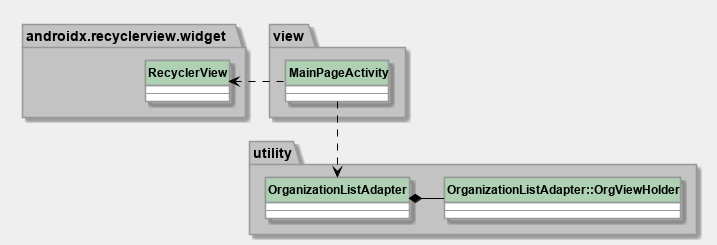
\includegraphics[width=6cm]{app-recyclerview.png}
  \caption{Diagramma delle classi per \java{RecyclerView}}
~~\label{fig:app/diagramma_classi_recyclerview}
\end{figure}

\subsubsection{Classe App}%
\label{subs:classe_app}

In alcune occasioni, ad esempio al momento della creazione della \java{RequestQueue} nel \java{WebSingleton} (§\ref{subs:richieste_http}), è necessario avere accesso al contesto dell'applicazione, rappresentato da un'istanza di \java{android.content.Context}.
Generalmente questo oggetto, condiviso da tutta l'applicazione, si ottiene invocando il metodo \java{getApplicationContext()} su una qualunque istanza di \java{Context} associata ad un'activity.
Per evitare di introdurre dipendenze circolari abbiamo scelto di definire la classe \java{utility.App}, derivata da \java{android.app.Application}, responsabile di mantenere lo stato globale dell'applicazione.
\java{App} ha un metodo aggiuntivo \java{getAppContext()} che espone direttamente il contesto dell'applicazione.

\subsubsection{Richieste HTTP}%
\label{subs:richieste_http}

Per le richieste HTTP abbiamo scelto la libreria \textit{Volley}, consigliata dalle guide ufficiali di Android, perché permette la loro esecuzione asincrona ed efficiente, senza la difficoltà associata alla gestione di un sistema di worker thread.
Le richieste vengono inserite in una struttura a coda gestita da un'istanza di \java{com.android.volley.RequestQueue}, la quale mantiene anche una cache.
Per questo motivo, l'efficienza della libreria migliora se tutte le richieste che l'app effettua sono convogliate nella stessa coda, quindi le guide suggeriscono di astrarre ulteriormente la funzionalità attraverso un singleton.
La classe \java{utility.web.WebSingleton} espone metodi per eseguire specifiche richieste HTTP al server di Stalker, come \java{login()} o \java{signup()}, ed il metodo \java{addToRequestQueue()} per effettuare una richiesta generica.

\paragraph{Autenticazione}%
\label{par:autenticazione}

Le richieste che richiedono l'autenticazione devono contenere un header \texttt{Authorization} contenente un JWT valido come valore.
La classe \java{utility.web.AuthenticatedRequest} aggiunge automaticamente questo header, utilizzando il decorator pattern.

\subsubsection{Gestione della posizione}%
\label{subs:gestione_della_posizione}

Per la raccolta delle informazioni sulla posizione, Stalker sfrutta le API esposte dalle librerie native di Android.
Abbiamo astratto le chiamate alle API grazie alla classe \java{GooglePositionInterface}.
Sono forniti i metodi:

\begin{itemize}
  \item \java{checkPermissions(Activity activity)} per verificare che l'utente abbia concesso i permessi di geolocalizzazione necessari all'app, ed eventualmente richiederli.
  \item \java{startLocationUpdates()} per iniziare a ricevere update sulla posizione
  \item \java{stopLocationUpdates()} per fermare gli update sulla posizione
\end{itemize}

\paragraph{Elaborazione della posizione}%
\label{par:elaborazione_della_posizione}

Le API di Android permettono di associare dei metodi callback all'arrivo di nuove informazioni sulla posizione.
Per l'elaborazione in background di queste informazioni, Stalker ha a disposizione la classe \linebreak\java{utility.location.LocationNotifier}, derivata da \java{androidx.core.app.JobIntentService}.
Essa raccoglie dei compiti da eseguire, rappresentati ciascuno da un contesto e da un'istanza di \java{android.content.Intent}, in una struttura a coda.
Ogni compito, quando raggiunge la cima della coda, viene eseguito invocando il metodo \linebreak\java{onHandleWork(Intent)}.

\paragraph{Geofences}%
\label{par:geofences}

Per ridurre il consumo di batteria, l'applicazione fa uso delle \textit{Geofences API} per attivare gli update sulla posizione solo se l'utente è nelle vicinanze di un luogo monitorato.
La classe \java{GeofencesHandler} mantiene l'elenco delle geofences attive, e sfrutta i \java{LiveData} per aggiornare le geofences ogni volta che l'utente si connette o disconnette da un'organizzazione.
La classe \java{GeofencesReceiver} è un \java{BroadcastReceiver} che riceve le notifiche relative all'entrata e all'uscita dalle geofences.
Mantiene l'elenco degli id dei luoghi nelle vicinanze dell'utente, e garantisce che gli update sulla posizione siano attivi se e solo se l'utente è nelle vicinanze di almeno un luogo.
% par:geofences (end)

\subsubsection{Sessione corrente}%
\label{subs:sessione_corrente}

Per mantenere le informazioni legate alla sessione corrente abbiamo scelto di utilizzare un singleton pattern, con la classe \java{utility.CurrentSessionSingleton}.
Per inserirsi nell'architettura MVVM, esso mantiene i propri campi dati in oggetti \java{androidx.lifecycle.MutableLiveData<T>}, al fine di implementare l'observer pattern.
Per prevenire le modifiche non controllate, espone getter che ritornano reference a \java{androidx.lifecycle.LiveData<T>}, che non permette l'aggiornamento dell'oggetto contenuto, ed espone metodi che permettono la modifica controllata dello stato dell'applicazione, come \java{setConnectedOrganization(int organizationId, boolean connected)} e \linebreak\java{updatePlaces(int organizationId,List<Place> places)}.
Inoltre, espone un metodo \java{getInsidePlaces(Point)} che ritorna la lista di \java{id} dei luoghi che contengono il punto passato come parametro fra tutti i luoghi monitorati, ciascuno associato al \java{id} della rispettiva organizzazione.
Infine, espone i metodi \linebreak\java{setUserOrganizationHistory(List<UserOrganizationHistory>)} e \java{getUserOrganizationHistory()} per accedere alla rappresentazione della cronologia sugli spostamenti dell'utente.

\subsubsection{Logica di business}%
\label{subs:logica_di_business}

Il subpackage \java{business} contiene le classi utilizzate per rappresentare i concetti prettamente legati a Stalker, come organizzazioni, luoghi, posizioni e utenti.
Queste classi fanno uso delle annotazioni del progetto \textit{Lombok} per generare automaticamente metodi come getter, setter, \java{toString()}, \java{equals()}.

\paragraph{LdapCredentials}%
\label{par:ldapcredentials}

La classe \java{LdapCredentials} rappresenta una coppia di credenziali LDAP da inviare al server.
Espone un metodo per la serializzazione a JSON\@.

% par:ldapcredentials (end)

\paragraph[Organization]{\java{Organization}}%
\label{par:app/organization}

La classe \java{Organization} espone un costruttore ad un parametro di tipo \java{org.json.JSONObject} utilizzato per costruire un'istanza a partire dalle risposte HTTP inviate dal server.
Inoltre, espone un metodo \java{getInsidePlaces(Point)} che ritorna la lista degli \java{id} dei luoghi che contengono il punto passato come parametro fra i luoghi legati all'organizzazione.

\paragraph[Place]{\java{Place}}%
\label{par:place}

La classe \java{Place}, in modo simile a \java{Organization}, espone un costruttore di tipo \java{org.json.JSONObject} utilizzato per costruire un'istanza a partire dalle risposte HTTP inviate dal server.
Inoltre, espone un metodo \java{isInside(Point)} che verifica se un dato punto è all'interno del luogo.
La verifica è eseguita utilizzando il calcolo vettoriale.
Per ogni vertice del poligono, sono definiti il vettore da esso al vertice successivo ed il vettore da esso al punto passato come parametro.
Sono poi calcolati i prodotti vettoriali: se tutti i prodotti vettoriali hanno lo stesso verso, il punto è all'interno, altrimenti è all'esterno.
Eventuali prodotti nulli indicano che i tre punti sono allineati.
È inoltre fornito un metodo \java{getCenter()} che ritorna il baricentro del poligono associato al place.

\paragraph[Point]{\java{Point}}%
\label{par:point}

La classe \java{Point} rappresenta un punto in coordinate cartesiane.
Espone un metodo statico \linebreak\java{buildFromDegrees(double longitude, double latitude)} per costruire un punto a partire dalle coordinate polari utilizzate in geolocalizzazione.
Per la conversione, abbiamo definito dei metodi privati che implementano la proiezione sferica di Mercatore e la rispettiva proiezione inversa.
Inoltre, \java{Point} implementa l'interfaccia \java{android.os.Parcelable} per la serializzazione e deserializzazione automatica da parte del sistema operativo.

\paragraph[User]{\java{User}}%
\label{par:app/user}

La classe \java{User} semplicemente raccoglie i dati dell'utente, ed espone un metodo per verificare che tutte le informazioni dell'utente siano presenti.

\paragraph[UserOrganizationHistory]{\java{UserOrganizationHistory}}%
\label{par:userorganizationhistory}

La classe \java{UserOrganizationHistory} rappresenta una entry nella cronologia dell'utente; espone un costruttore per deserializzare i corrispettivi oggetti JSON ottenuti dal server.

% par:userorganizationhistory (end)

\end{document}
